\documentclass[a4paper,11pt,oneside]{book}
\usepackage{pgfplots}

\begin{document}

\subsection*{Figure 1.1}
\begin{tikzpicture}
\begin{axis}[
    axis lines = left,
    xlabel = $t\;(s)$,
    ylabel = {$v\;(m/s)$},
]
%Below the red is defined
\addplot [
    domain=0:40, 
    samples=100, 
    color=red,
]
{20};
\addlegendentry{$Cay\;X$}

%Here the blue is defined
\addplot [
    domain=0:40, 
    samples=100, 
    color=blue,
]
{x};
\addlegendentry{$Car\;Y$}

\end{axis}
\end{tikzpicture}

\subsection*{Figure 1.2}
\begin{tikzpicture}

\begin{axis}[
    axis lines = left,
    xlabel = $t\;(s)$,
    ylabel = {$v\;(m/s)$},
]

%Below the black is defined
\addplot [
    domain=5:100,
    samples=100, 
    color=black,
]
{0.3};
\addlegendentry{terminal velocity}
%Below the red is defined
\addplot [
    domain=0:100,
    range=0:2,
    samples=100, 
    color=red,
]
{x/(10+3.333*x)};

%Below the black is defined
\addplot [
    domain=1:100,
    samples=100, 
    color=white,
]
{0.5};

\end{axis}
\end{tikzpicture}

\subsection*{Figure 1.3}
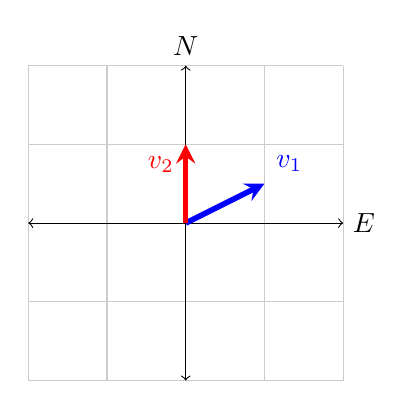
\begin{tikzpicture}
  \draw[thin,gray!40] (-2,-2) grid (2,2);
  \draw[<->] (-2,0)--(2,0) node[right]{$E$};
  \draw[<->] (0,-2)--(0,2) node[above]{$N$};
  \draw[line width=2pt,blue,-stealth](0,0)--(1,0.5) node[anchor=south west]{$v_1$};
  \draw[line width=2pt,red,-stealth](0,0)--(0,1) node[anchor=north east]{$v_2$};
\end{tikzpicture}

\subsection*{Figure 1.4}
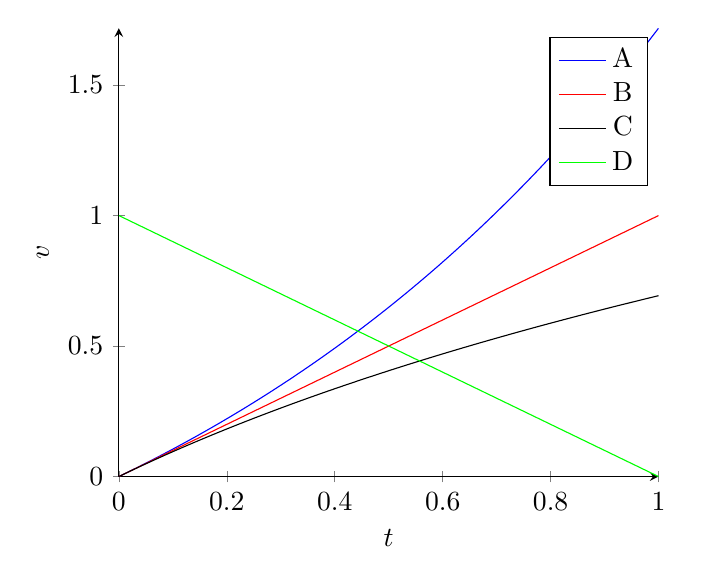
\begin{tikzpicture}
\begin{axis}[
    axis lines = left,
    xlabel = $t$,
    ylabel = {$v$},
]

%A
\addplot [
    domain=0:1,
    samples=100, 
    color=blue,
]
{e^x-1};
\addlegendentry{A}

%B
\addplot [
    domain=0:1,
    samples=100, 
    color=red,
]
{x};
\addlegendentry{B}

%C
\addplot [
    domain=0:1,
    samples=100, 
    color=black,
]
{ln(x+1)};
\addlegendentry{C}

%D
\addplot [
    domain=0:1,
    samples=100, 
    color=green,
]
{1-x};
\addlegendentry{D}

\end{axis}
\end{tikzpicture}
\end{document}
